%C, C\#, C++, Java, UNIX shell scripting, Windows CMD line scripting, GNU make, SQL (MySQL, Microsoft SQL Server 2000-current), CUDA, OpenMP, OpenCL, OpenGL, MPI, Gridgain, CSS, XML, XHTML, HTML, and others
%C, C++, Java, UNIX shell scripting, Windows CMD line scripting, CUDA, OpenMP, OpenCL, and others

\documentclass[tikz,border=2mm]{standalone}

\begin{document}
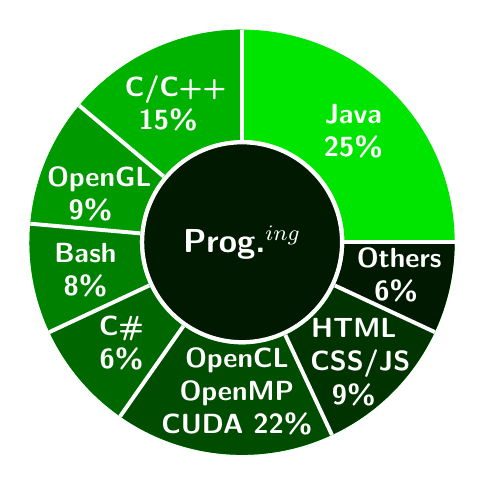
\begin{tikzpicture}[font=\sffamily\bfseries\large, 
     text=white, 
     border/.style={line width=14mm}]
\foreach \angle/\col [remember=\angle as \last (initially 0)] in 
    {360/green!90!black, 335/green!10!black, 295/green!20!black, 235/green!30!black, 205/green!40!black, 175/green!50!black, 140/green!60!black, 90/green!70!black, 90/green!90!black}{    
		\draw[\col, border] (\last:2cm) 
             arc[start angle=\last, end angle=\angle, radius=2cm];
		\draw[white, line width=0.5mm] (\last:1.3)--++(\last:1.4);
}
\node[text width=1.5cm, align=center, font=\sffamily\bfseries\large, draw, circle, minimum width=2.5cm, white, fill=green!10!black] {Prog.$^{ing}$};
\node[text width=1.1cm, align=center, font=\sffamily\bfseries\normalsize] at (45:2cm) 
    {Java 25\%};
\node[text width=1.1cm, align=center, font=\sffamily\bfseries\normalsize] at (118:2cm) 
    {C/C++ 15\%};
\node[text width=1.1cm, align=center, font=\sffamily\bfseries\normalsize] at (162.5:2.02cm) 
    {OpenGL 9\%};    
\node[text width=1.1cm, align=center, font=\sffamily\bfseries\normalsize] at (190:2.02cm) 
    {Bash 8\%};  
\node[text width=1.1cm, align=center, font=\sffamily\bfseries\normalsize] at (220:2cm) 
    {C\# 6\%};       
\node[text width=3.0cm, align=center, font=\sffamily\bfseries\normalsize] at (268:1.9cm) 
    {OpenCL \\ OpenMP \\ CUDA 22\%};
\node[text width=1.1cm, align=center, font=\sffamily\bfseries\normalsize] at (313:2.08cm) 
    {HTML CSS/JS 9\%};
\node[text width=1cm, align=center, font=\sffamily\bfseries\normalsize] at (348:2cm) 
    {Others \\ 6\%};
\end{tikzpicture}
\end{document}
